\section{相关工作}
\label{sec:related_work}

\begin{figure*}
	\centering
	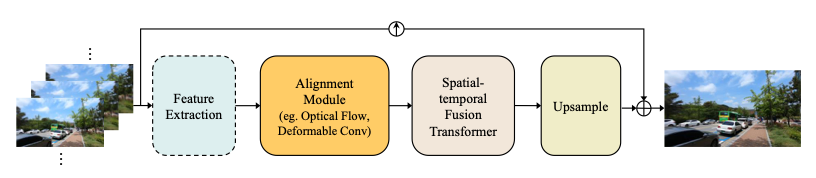
\includegraphics[width=\linewidth]{6.png}
	\caption{VSR 网络模块示意图}
	\label{fig:fig6}
\end{figure*}

\begin{table*}[!t]
\caption{Components in existing VSR methods. }
	\begin{center}
		\tabcolsep=0.1cm
		\scalebox{0.9}{
			\begin{tabular}{l|c|c|c|c|c|c|c|c}
				\hline
				\multirow{2}{*}{} & \multicolumn{3}{c|}{Sliding-Window} & \multicolumn{5}{c}{Recurrent}                                                                                                                                                                                                            \\ \cline{2-9}
				%
				                  & EDVR      & MuCAN      & TDAN & BRCN & FRVSR  & RSDN  & \textbf{\mbox{BasicVSR}} & \textbf{\mbox{IconVSR}}          \\ \hline
				%
				Propagation       & Local                               & Local                         & Local                    & \textbf{Bidirectional}                            & Unidirectional                & Unidirectional              & \textbf{Bidirectional}   & \textbf{Bidirectional} (coupled) \\
				Alignment         & \textbf{Yes} (DCN)                  & \textbf{Yes} (correlation)    & \textbf{Yes} (DCN)       & No                                                & \textbf{Yes} (flow)           & No                          & \textbf{Yes} (flow)      & \textbf{Yes} (flow)              \\
				Aggregation       & Concatenate + \textbf{TSA}          & Concatenate                   & Concatenate              & Concatenate                                       & Concatenate                   & Concatenate                 & Concatenate              & Concatenate + \textbf{Refill}    \\
				Upsampling        & Pixel-Shuffle                       & Pixel-Shuffle                 & Pixel-Shuffle            & Pixel-Shuffle                                     & Pixel-Shuffle                 & Pixel-Shuffle               & Pixel-Shuffle            & Pixel-Shuffle                    \\ \hline
			\end{tabular}}
		\vspace{-0.3cm}
	\end{center}
\end{table*}

\begin{figure}[!htbp]
\vspace{-5mm}
  \centering
  \begin{minipage}[b]{\linewidth} 
    \subfloat[]{
    \begin{minipage}[b]{0.25\linewidth}
      \centering
      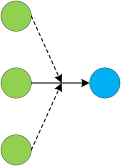
\includegraphics[width=\linewidth]{5-1.png}
     \end{minipage}
  }
  \hspace{5mm}
   \subfloat[]{
    \begin{minipage}[b]{0.25\linewidth}
      \centering
      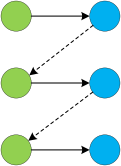
\includegraphics[width=\linewidth]{5-2.png}
     \end{minipage}
  }
   \hspace{5mm}
  \subfloat[]{
    \begin{minipage}[b]{0.25\linewidth}
      \centering
      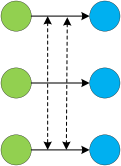
\includegraphics[width=\linewidth]{5-3.png}
     \end{minipage}
  }
      \end{minipage}
  \caption{VSR 网络架构示意图:(a) Sliding-Window;(b) Recurrent;(c) Transformer}
  \label{fig:fig5}
\end{figure}

在 BasicVSR 中,作者将 VSR 网络分为4个功能块 Propagation、Alignment、Aggregation(Fusion)、Upsampling,如 \textbf{图 \ref{fig:fig6}} 所示,针对 VSR 的网络设计也主要是从这四个方面入手。如 \textbf{图 \ref{fig:fig5}} 所示,根据 VSR 利用视频序列信息的方式,可以将现有网络分为Sliding-Window和Recurrent两类。而近期一些工作受 Transformer 模型对序列数据并行计算能力的驱动,将该模型引入到了 VSR 任务中。本文研究的出发点就在于 Transformer 模型对齐模块的设计。

局部性归的纳偏置指的是 CNN 只能看到当前和附近的位置,如 \textbf{图 \ref{fig:fig7}},在 $T_1$ 帧的时候,物体还在画面的右上角,但是到了 $T_2$ 它就往左下角移动了,如果直接将两帧叠在一起输入 CNN,网络根本没有办法利用到 $T_2$ 帧的信息。而在网络中引入 Alignment后,网络会把不同帧的物体挪到相同位置,使得网络可以在一个卷积核里面看到同一个物体在两帧里面的两个版本。

Alignment 基本上是之前所有 VSR 网络必备的模块。自 ViT 之后,Transformer 席卷了整个计算机视觉领域,2021年之后几个效果非常好的 SISR 方法基本上都是基于Transformer的。Transformer 有这么几个特性,例如把输入信号看作离散的token,使用多头自注意力在不同的token之间进行交互等,这些特性使得它非常适合拿来做长程依赖关系的建模。

\begin{figure}[!tbp]
\centering
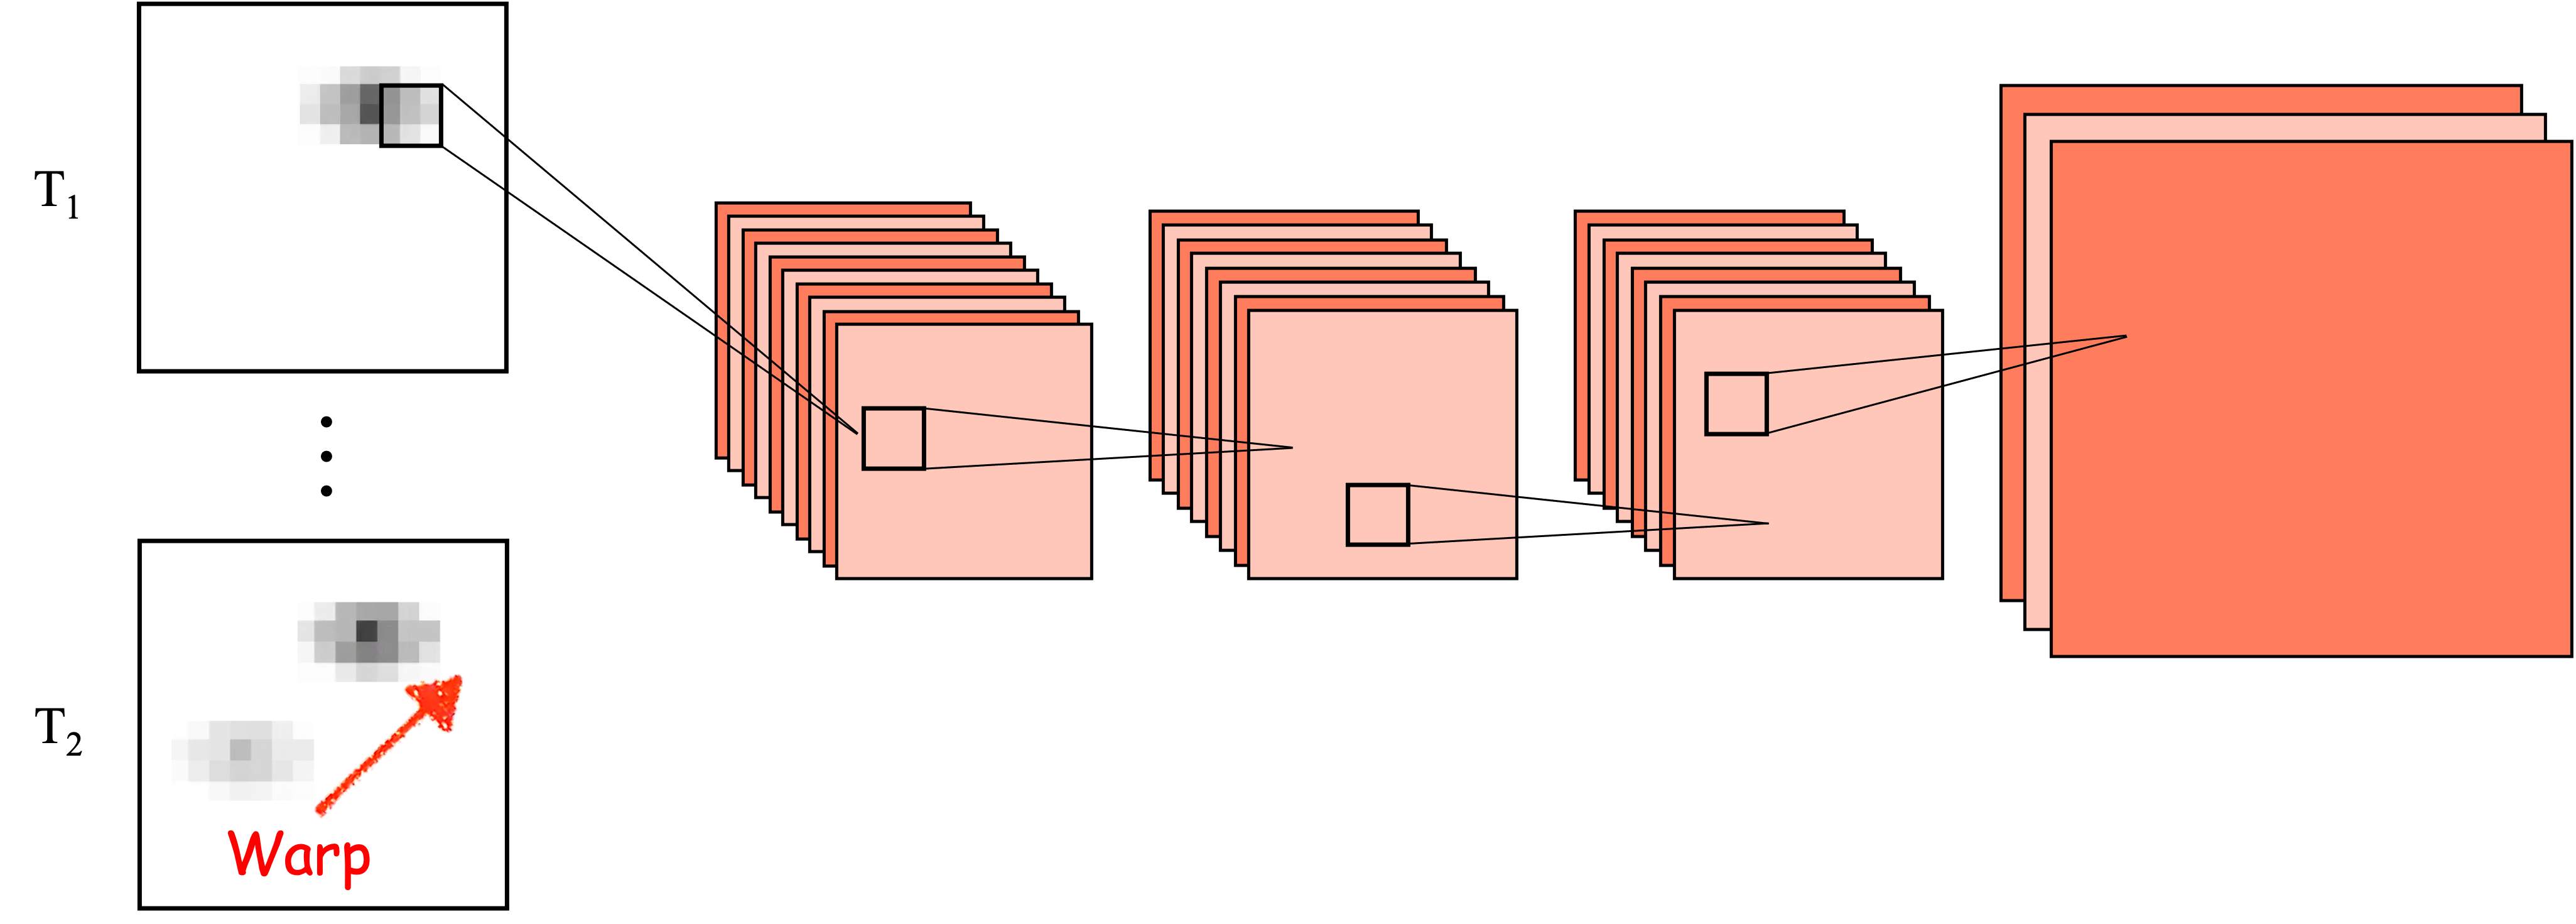
\includegraphics[width=\linewidth]{7.png}	
\caption{卷积神经网络的局部归纳偏置}
\label{fig:fig7}
\end{figure}

第一个特性就是它不像 CNN 是使用卷积或者滤波器去处理相邻两个像素或者甚至是更多像素之间的关系,Transformer 实际上是把输入信号看作一个一个离散的 token,然后他对空间上的交互或者说元素之间的交互是在token之间进行。在图像处理中,已经有很多工作表明比较高效的方法是把每一个像素都当做一个token。Transformer利用自注意力或者多头自注意力在不同的像素token之间进行交互。自注意力的特性是它非常适合拿来做长程的依赖关系或者分布关系的建模。如 \textbf{图 \ref{fig:fig8}} 所示,绿色的像素和红色的像素距离比较接近,但是绿色像素和蓝色像素离得比较远,在Transformer中,自注意力对他们的计算是一样的,也就是说绿色和红色的计算和绿色和蓝色这两套计算都服从同一套权重的计算方法。所以说对于Transformer来说,它处理绿色和红色和它处理绿色和蓝色没有任何的不同,虽然空间上二者关系并不一样,但是它去处理起来是没有区别的,即图中的两个箭头实际上是等价的。

\begin{figure}[!htbp]
\centering
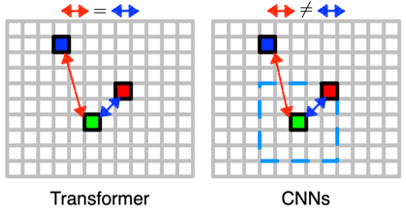
\includegraphics[width=\linewidth]{8.png}	
\caption{卷积神经网络和 Transformer 像素交互示意图}
\label{fig:fig8}
\end{figure}

但是 CNN 就不太一样了,以感受野为 $5 \times 5$ 的卷积为例,对于以绿色像素为中心的卷积操作,红色的像素是在卷积操作的感受野里,所以绿色像素和红色像素是可以在同一层直接进行交互的。但是蓝色的像素并不在这个卷积操作的感受野里面,要是使得绿色的像素和蓝色的像素进行交互,可能要经过多个 CNN 的卷积层,卷积操作的感受野才能作用到那边。此外,即使二者可以在同一个卷积操作的感受野中进行交互,其作用的强度和方法也是不一样的。

CNN 的感受野虽然有那么大,但是并不是感受野里面所有的元素都有同样的权重。越靠近中心的位置,它的权重越大,也就是网络对这个信息利用得越好,而越远离网络对信息利用的越不好。这就是为什么 CNN 会有一个局部性的归纳偏置。而对于视频超分辨率重建而言,只要这个物体挪开了,而且当挪得越远时,网络对信息的利用就越不好。

\begin{figure*}[!hb]
	\centering
	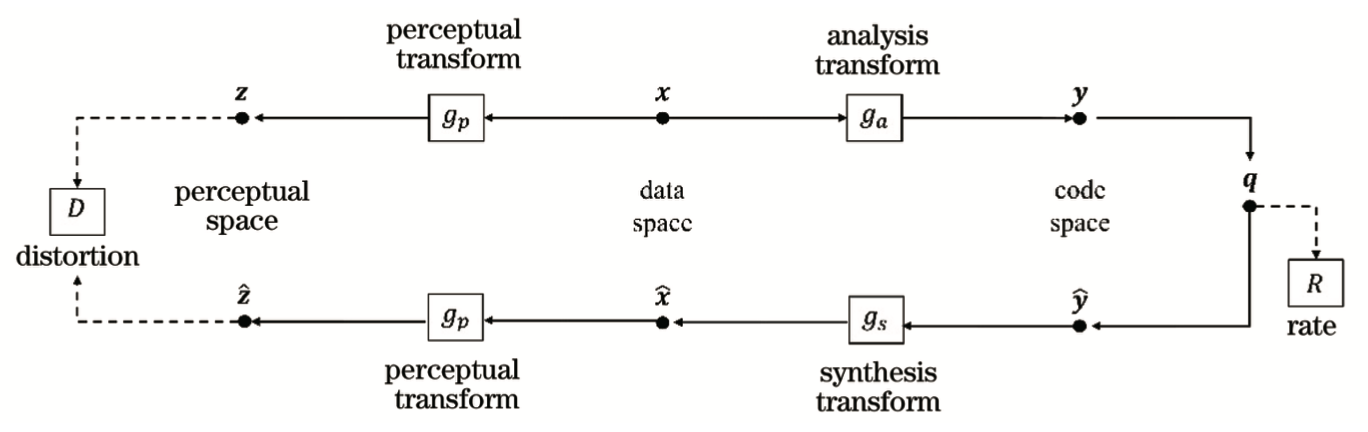
\includegraphics[width=\linewidth]{4.png}
	\caption{亚像素信息示意图}
	\label{fig:fig3}
\end{figure*}

同样,近年来 Transformer 在 VSR 领域的研究也发展迅速。例如减少模型的参数量、在频率域消除压缩伪影的影响等。
